\documentclass[10.5pt]{article}
\usepackage[a4paper,margin=2.1cm]{geometry}
\usepackage{amsmath,amssymb}
\usepackage{booktabs}
\usepackage{graphicx}
\usepackage[hidelinks]{hyperref}
\usepackage{enumitem}
\usepackage{caption}
\usepackage{float}
\setlist{itemsep=1pt,topsep=2pt}
\captionsetup{font=small,labelfont=bf}
\newcommand{\code}[1]{\texttt{#1}}
\emergencystretch=3em
\hypersetup{pdftitle={GStar Assignment 2: GRPO},pdfauthor={Phung Gia Huy}}

\title{\textbf{GStar Assignment 2: GRPO}}
\author{Phung Gia Huy}
\date{November 2026}

\begin{document}
\maketitle
\vspace{-10pt}
\begin{center}\small
Code: \url{https://github.com/huypg-zenai/GStar-Assignment-2-GRPO} \quad Runs: W\&B project \code{gstar-a2-grpo}
\end{center}

\paragraph{Summary.}
\begin{itemize}
\item All four RL runs beat the 37\% target: GRPO 58.5\% / 52.1\% and Dr.GRPO \textbf{60.7\%} / \textbf{55.9\%} at
  $L_{256}$ / $L_{512}$.
\item RL exploited the verifier: 13--17\% of ``correct'' $L_{256}$ answers leave numbers unused. Under the task's
  real rule the runs score 48--55\%.
\item GRPO tends to commit to wrong answers, Dr.GRPO to run out of tokens. We attribute this to GRPO's std
  normalisation amplifying the 0.1 partial credit.
\item \textbf{Problem 2} applies the same pipeline to poker decisions graded by an exact game solution. An exact reward cuts
  exploitability by 30\% and generalises to unseen situations; a noisy reward improves, then degrades. The trained
  model picks better actions, but its stated reasons are \emph{less} often correct than before training.
\end{itemize}

\section{Implementation and setup}
\textbf{Tasks 1--5} are in \code{starter.py}; \code{tests/} checks every handout example plus edge cases (20 tests pass).
\code{\_extract\_answer} takes the last \code{<answer>} tag; \code{\_validate\_numbers} checks the numbers form a
sub-multiset of those given (as specified); \code{\_evaluate\_equation} allows only digits, spaces, \code{+-*/()} and
returns \code{None} on any error. \code{reward\_fn} gives 0 (no tag), 0.1 (tag but wrong) or 1.0. Advantages are
$r-\bar r$, divided by $\mathrm{std}+\epsilon$ for GRPO only. The loss is the per-token PPO clipped surrogate.
\code{masked\_mean} averages per sequence then over the batch; \code{masked\_mean\_drgrpo} sums per sequence and
divides by a constant \code{num\_tokens}.

\textbf{Setup.} We trained on Kaggle's free 2$\times$T4 GPUs instead of an A100. That forced fp16 (no bf16 on T4) and
LoRA ($r=\alpha=32$) instead of full fine-tuning, with vLLM generating on the second GPU. Merged weights are synced into
vLLM every step; vLLM's and the policy's log-probs of the sampled tokens differ by only 0.001--0.005 nats/token, so
rollouts are on-policy. All runs: 80 steps, 128 rollouts per step (16 prompts $\times$ 8), lr $5\times10^{-5}$,
$\epsilon=0.2$, temperature 1.0, evaluation on the 1,024 test prompts every 10 steps.

\section{Conceptual questions}
\textbf{Clipping: on- or off-policy?} Off-policy. Clipping acts only when $\rho_t=\pi_\theta/\pi_{\theta_\text{old}}$ leaves
$[1-\epsilon,1+\epsilon]$. On-policy, the rollouts come from the parameters being updated, so $\rho_t=1$ and the loss is the
plain policy gradient. That is our case: \code{starter.py} sets \code{old\_log\_probs = policy\_log\_probs.detach()} and
takes one optimiser step per batch, so the clip never fires. When data is reused after the policy changes (several
epochs, stale or asynchronous rollouts), $\rho_t$ drifts, and the clip stops a few high-advantage tokens from pushing the
policy far from where the data was collected.

\textbf{On-policy advantages:} (1) an unbiased gradient with no importance weights or $\epsilon$ to tune; (2) the baseline
reflects current behaviour, which changes fast here (length falls by a third in 30 steps at $L_{256}$).
\textbf{Off-policy advantages:} (1) sample efficiency: generation costs 15--33\,s per step, and early on 86--89\% of
$L_{256}$ groups carry no signal, so reusing the rare successes is valuable; (2) generation and training can run in
parallel on the two GPUs with slightly stale weights, instead of waiting for each other.

\textbf{Gradients under the two reductions.} We ran the handout's batch through our \code{compute\_loss} and both reductions
and called \code{backward()} (\code{report/grad\_reductions.py}; $\rho=1$, same advantage $A$, $B=2$, \code{num\_tokens}=6):
\begin{center}\small
\begin{tabular}{lccc}
\toprule
Reduction & per short-response token & per long-response token & total weight, short / long\\
\midrule
\code{masked\_mean} & $-0.167A$ & $-0.083A$ & $-0.5A$ / $-0.5A$\\
\code{masked\_mean\_drgrpo} & $-0.083A$ & $-0.083A$ & $-0.25A$ / $-0.5A$\\
\bottomrule
\end{tabular}
\end{center}
\code{masked\_mean} weights each \emph{response} equally, so short responses get twice the per-token gradient.
\code{masked\_mean\_drgrpo} weights each \emph{token} equally, so a response's weight grows with its length. With $A<0$,
\code{masked\_mean} penalises long wrong answers less per token. This is the length bias that lets wrong answers grow.
\emph{Prefer \code{masked\_mean}} when lengths vary widely and each sample should count equally, for example a few very long
truncated rollouts that would otherwise dominate the update. \emph{Prefer \code{masked\_mean\_drgrpo}} for long
chain-of-thought, where the length bias inflates wrong answers. Our $L_{512}$ runs fit this: Dr.GRPO is shorter (356 vs
374 tokens) and more accurate.

\section{Problem 1: results and analysis}
\begin{table}[H]
\centering\small
\resizebox{\linewidth}{!}{%
\begin{tabular}{llccccc}
\toprule
Model & Max tokens & Accuracy & Strict acc.$^\dagger$ & Correct / partial / failed & Avg tokens & Best eval (step)\\
\midrule
Zero-shot & $L_{256}$ / $L_{512}$ / $L_{1024}$ & 0.0 / 9.0 / 8.7\% & same & see Fig.~\ref{fig:failures} & 256 / 498 / 888 & --\\
GRPO & $L_{256}$ & 58.5\% & 48.4\% & 599 / 310 / 115 & 139 & 58.5\% (80)\\
Dr.GRPO & $L_{256}$ & \textbf{60.7\%} & \textbf{52.9\%} & 622 / 36 / 366 & 161 & 61.1\% (70)\\
GRPO & $L_{512}$ & 52.1\% & 51.9\% & 533 / 10 / 481 & 374 & 52.1\% (70)\\
Dr.GRPO & $L_{512}$ & \textbf{55.9\%} & \textbf{55.3\%} & 572 / 10 / 442 & 356 & 55.9\% (80)\\
\bottomrule
\end{tabular}}
\caption{Accuracy on the 1,024 test prompts after 80 steps. Partial = reward 0.1, failed = 0.
$^\dagger$Correct \emph{and} using every number, as the task requires.}
\label{tab:p1}
\end{table}

\begin{figure}[H]
\centering
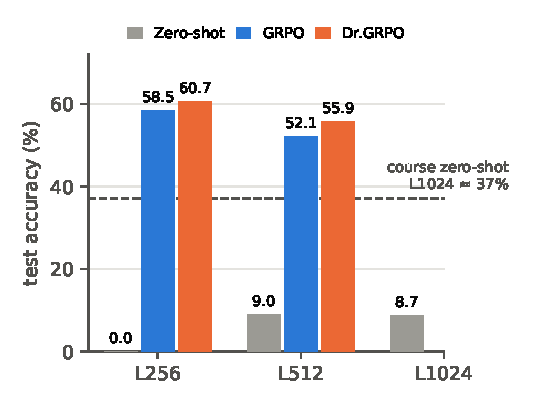
\includegraphics[width=0.49\linewidth]{figures/p1_accuracy.pdf}\hfill
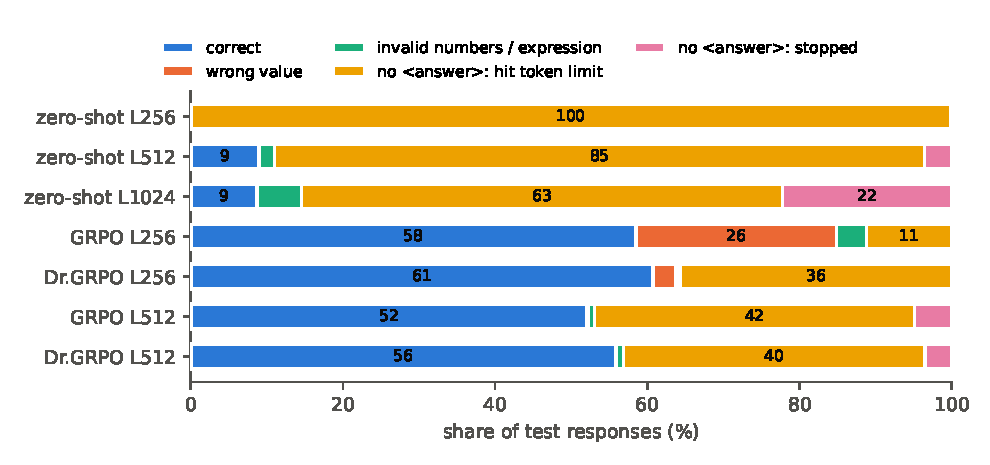
\includegraphics[width=0.49\linewidth]{figures/p1_failures.pdf}
\caption{Left: final accuracy; the dashed line is the course's zero-shot $L_{1024}$ reference. Right: how every test
response ends, using the reward's own verifier functions (\code{report/analyze\_p1.py}).}
\label{fig:failures}
\end{figure}

\begin{figure}[H]
\centering
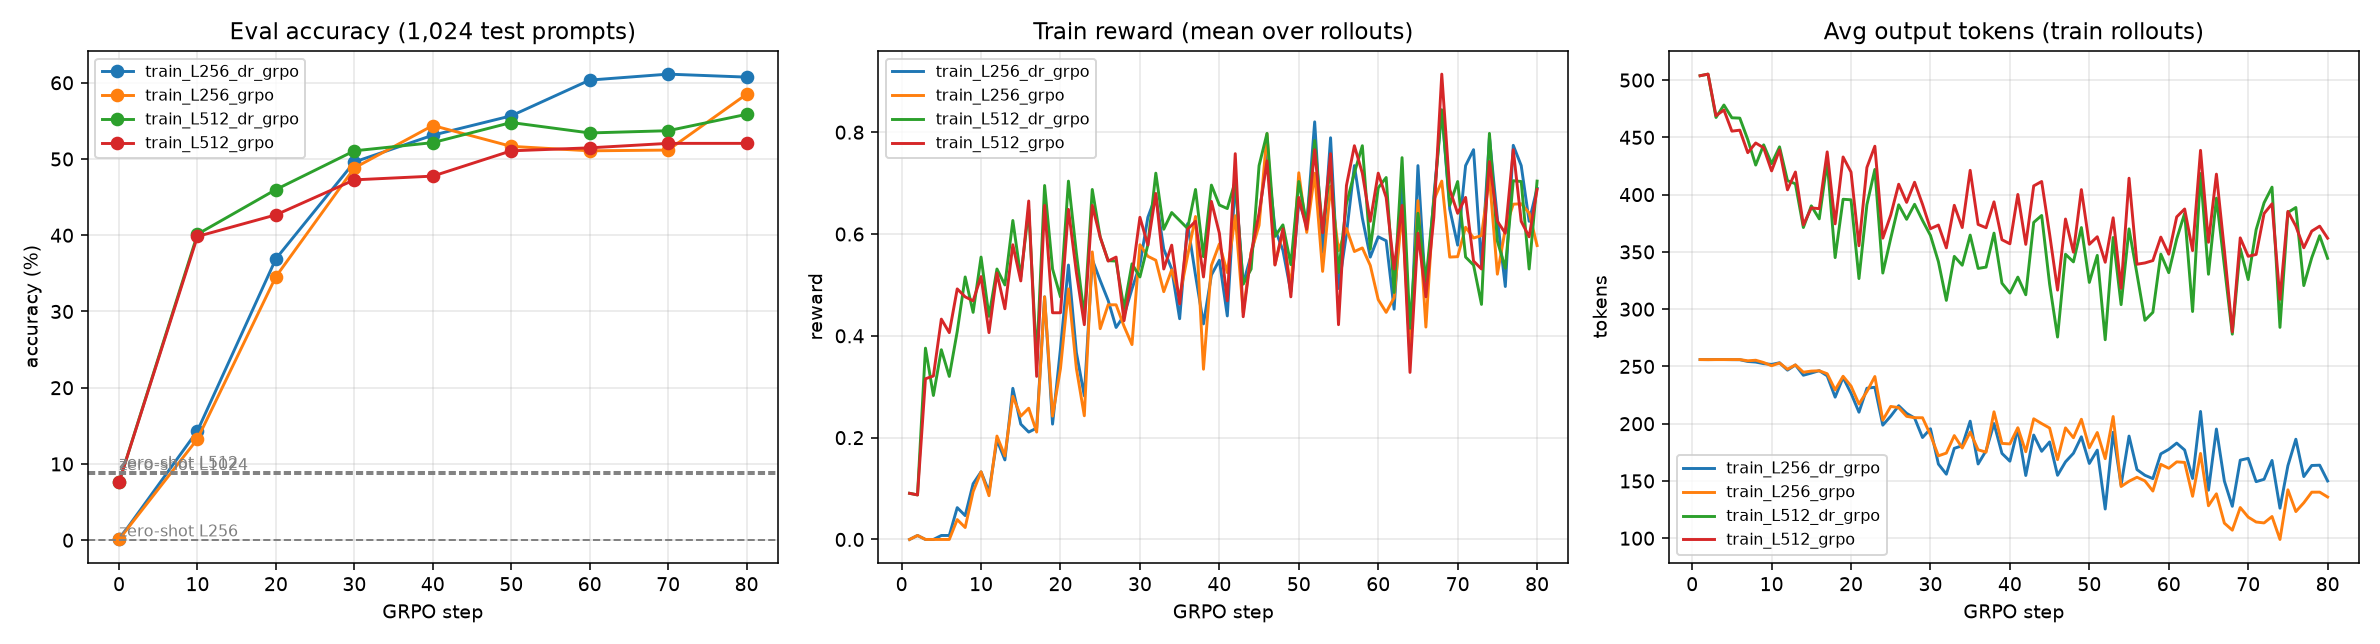
\includegraphics[width=\linewidth]{figures/p1_curves.png}
\caption{Training curves: test accuracy, mean training reward and output length. No run became unstable within 80 steps.}
\label{fig:curves}
\end{figure}

\paragraph{Zero-shot is below the handout's numbers} (ours 0.0 / 9.0 / 8.7\% vs 0.1 / 15 / 37\%), although prompt,
sampling and scoring match \code{zero\_shot\_eval.py} and the model weights are unchanged since release. At $L_{1024}$,
63\% of answers hit the limit (often in loops such as ``45. 45. 45.'') and 22\% stop without a tag, which caps accuracy
at 37\%. We suspect fp16 (forced by the T4s) makes long samples loop more often, but could not test bf16. Every run,
baseline included, uses the same precision, so the RL comparison is unaffected.

\paragraph{What worked.}
\begin{itemize}
\item \textbf{Most of the gain is learning to finish.} Zero-shot is cut off on 100\% ($L_{256}$) and 85\% ($L_{512}$) of
  answers. RL shortens $L_{256}$ answers from 256 to 139--161 tokens, into quick trial-and-error searches
  (``79 $-$ 60 = 19, 17 + 19 = 36! \code{<answer>17 + (79 - 60)</answer>}'').
\item \textbf{Easy instances are solved.} Accuracy on 3-number problems is 79--84\% in every run, against 27--40\% on
  4-number problems, which need nested expressions the greedy search rarely finds.
\item \textbf{Dr.GRPO beats GRPO at both lengths} (+2.2 and +3.8 points) and is still improving at step 80 at $L_{512}$.
\end{itemize}

\paragraph{What failed, and why.}
\begin{itemize}
\item \textbf{Reward hacking.} The verifier (as specified) accepts any \emph{subset} of the numbers. RL found this: 17\%
  (GRPO) and 13\% (Dr.GRPO) of correct $L_{256}$ answers skip numbers, for example \code{55 + 38} for target 93 with
  [55, 38, 69, 68]. Zero-shot never does this, and the $L_{512}$ runs rarely do. Under the strict rule, $L_{512}$ beats
  $L_{256}$ for both methods.
\item \textbf{GRPO guesses; Dr.GRPO runs out of tokens} ($L_{256}$: 26\% vs 3\% wrong values; 11\% vs 36\% truncated).
  GRPO also learned an empty \code{<think></think>} and does its search outside it. \emph{Hypothesis:} in groups with no
  correct answer, rewards are 0 (truncated) or 0.1 (any answer). GRPO divides by their small std, so ``write some answer''
  earns advantages near $\pm1$, as large as solving the problem. Dr.GRPO keeps this signal at $\le0.1$.
\item \textbf{$L_{512}$ still truncates 40--42\%}, but almost never gives a wrong value (0--2 answers): its problem is
  finishing, not accuracy.
\end{itemize}

\paragraph{Improvements.} (1) Require every number exactly once in the verifier. (2) Drop the 0.1 partial credit once the
format is learned, or give it only to answers that use all numbers. (3) Skip groups with identical rewards (38--68\% of
groups late in training). (4) Use a soft length penalty or an $L_{256}\to L_{512}$ curriculum instead of hard truncation.
(5) Retest the zero-shot gap on bf16 hardware.

\section{Problem 2 (extra credit): reasoning about poker with GRPO}
\paragraph{Question.} Countdown has one right answer per prompt. Many real decisions do not: the best action depends on
hidden information and on other agents. \textbf{Can GRPO teach Qwen3-1.7B to reason in such a setting, and does the reward
design matter when feedback is noisy?}

\paragraph{Setup.} \emph{Leduc Hold'em}: a 6-card deck (J J Q Q K K), one private and one public card, two betting rounds,
only 288 decision points. That is small enough to solve exactly with CFR+ and to compute the \textbf{exploitability} of any
strategy: chips per hand a perfect adversary wins against it (0 = equilibrium). Our engine matches OpenSpiel's
\code{leduc\_poker} to 6 decimals. Each prompt is one decision in plain English; the model reasons briefly and answers with
one action in \code{<answer>} tags. Training situations come half from equilibrium self-play and half uniformly at random;
\textbf{90 of the 288 situations are held out} to test generalisation. Code, GPUs and hyper-parameters are those of
Problem 1 ($L_{512}$, 80 steps).

\paragraph{Two rewards} (a legal action scores $0.1+0.9\cdot$score, otherwise 0):
\code{ev} scores the action's exact value under the equilibrium (no noise); \code{outcome} plays the hand out \emph{once}
and scores the chips won. On average they are equal; \code{outcome} is just noisy (std about 4 chips against value
gaps of 1--3).

\paragraph{Hypotheses, written before running.} \textbf{H1}: RL lowers exploitability and generalises to held-out
situations. \textbf{H2}: the noisy reward learns worse with the same compute. \textbf{H3}: because the reward assumes a
fixed opponent, the policy stops mixing its actions, so high reward will not mean equilibrium play.

\paragraph{Evaluation.} The model answers every one of the 288 situations $k$ times ($k=8$ for zero-shot and the final
models, 2 during training); the answers form a strategy that is scored exactly, with no sampled games.

\paragraph{Pilot.} With Qwen3's thinking mode, every rollout hit the 512-token limit (0.04\% valid answers), so every
reward was 0 and the gradient was exactly 0. Turning thinking off and asking to ``think briefly (a few sentences)'' gave
95.8\% valid answers and 0\% truncation. The training script now aborts if fewer than 5\% of step-0 answers are valid.

\begin{table}[H]
\centering\small
\resizebox{\linewidth}{!}{%
\begin{tabular}{lcccccccc}
\toprule
Policy & Expl.\,$\downarrow$ & vs eq. & vs raise-bot & EV reward & seen & held-out & Regret\,$\downarrow$ & Tokens\\
\midrule
Always check/call / uniform random & 1.47 / 2.37 & $-0.63$ / $-0.70$ & -- & -- & -- & -- & -- & --\\
Zero-shot Qwen3-1.7B & 3.13 & $-0.56$ & $-1.53$ & 0.641 & 0.652 & 0.617 & 1.55 & 140\\
GRPO, \code{ev} reward & \textbf{2.18} & $-0.15$ & $-0.78$ & \textbf{0.860} & \textbf{0.882} & \textbf{0.811} & \textbf{0.29} & 64\\
GRPO, \code{outcome} reward & 3.76 & $-0.15$ & $-2.29$ & 0.756 & 0.801 & 0.657 & 0.39 & 54\\
\bottomrule
\end{tabular}}
\caption{Final models ($k=8$). Exploitability and ``vs'' columns in chips per hand; regret in chips per decision.}
\label{tab:p2}
\end{table}

\begin{figure}[H]
\centering
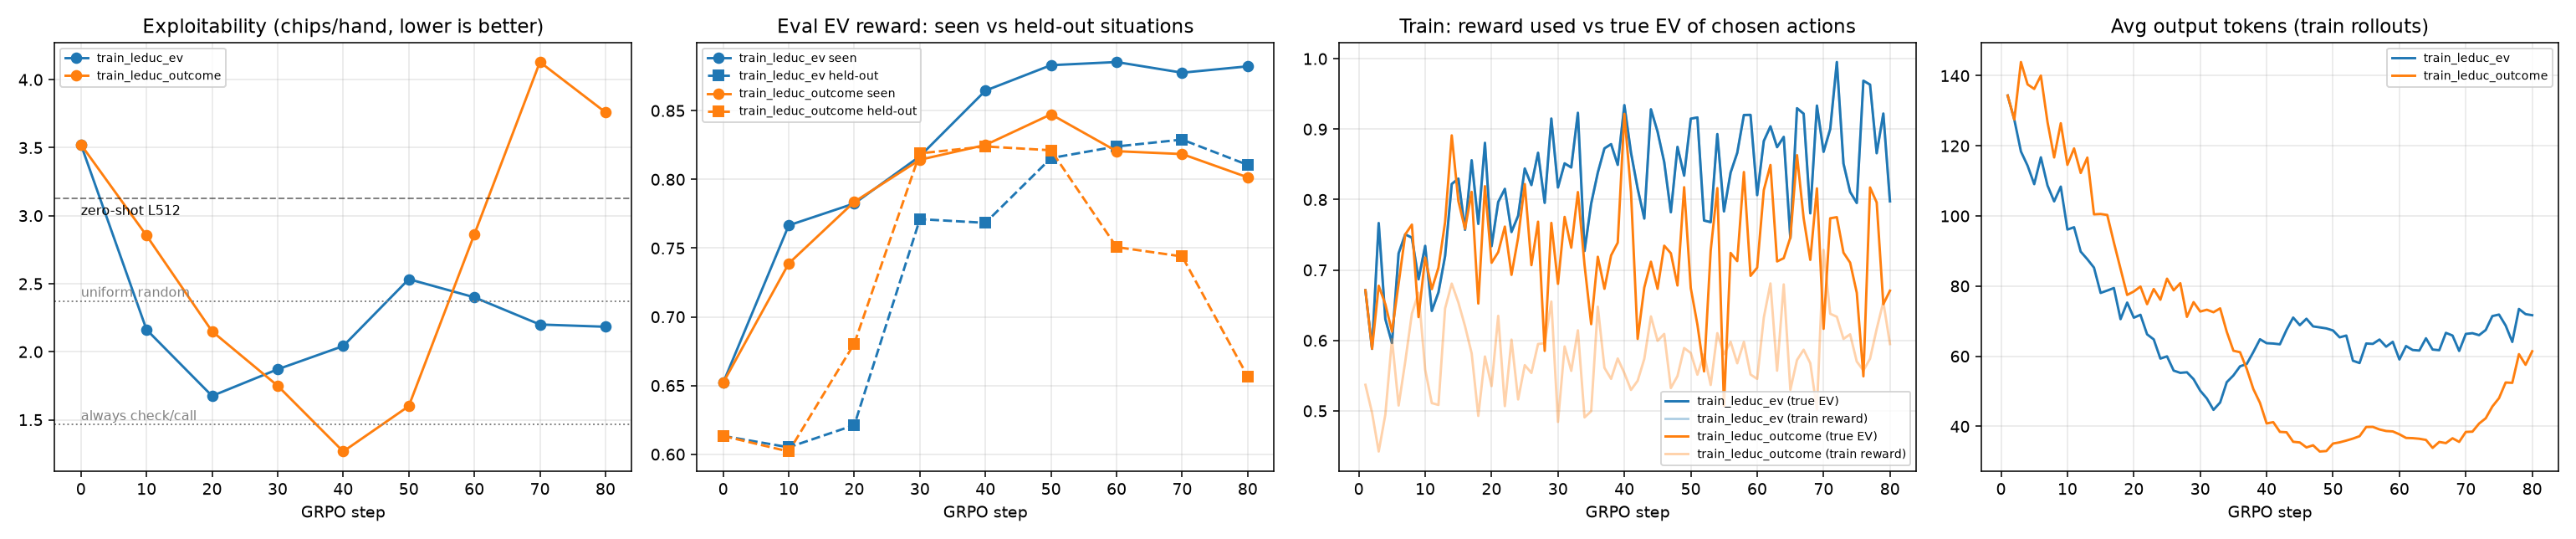
\includegraphics[width=\linewidth]{figures/p2_curves.png}
\caption{Training: exploitability; EV reward on seen (solid) vs held-out (dashed) situations; training reward (faint) vs
true EV of the chosen actions; output length. Evals before step 80 use $k=2$ and are noisy.}
\label{fig:p2}
\end{figure}

\paragraph{H1 holds with the exact reward.} Exploitability falls 30\% (3.13 $\to$ 2.18) and regret 81\%. Held-out EV rises
almost as much as seen EV (0.617 $\to$ 0.811 vs 0.652 $\to$ 0.882), although those situations were never trained on.
For example, facing a bet with a pair it now always calls, where zero-shot folded up to 60\% of the time.

\paragraph{H2 holds, more strongly than expected.} The noisy reward improves until about step 40 and then degrades. It
ends \emph{more} exploitable than zero-shot (3.76) and drifts into raising 89\% of the time (equilibrium: 39\%). The
reward it trains on stays flat at about 0.55--0.60 while the true value of its actions moves underneath
(Fig.~\ref{fig:p2}, panel 3). With 80 steps $\times$ 16 situations, the updates follow noise as much as signal.

\paragraph{H3 holds: reward is not the objective.} In the \code{ev} run, entropy where the equilibrium mixes collapses from
0.64 to 0.06, so the policy stops bluffing. Exploitability is lowest at step 20 (1.68) and then rises to about 2.2 while the
EV reward keeps climbing. The final policy is a \emph{calling station}: it folds to 22\% of bets (equilibrium: 42\%) and
bets or raises 27\% of the time (39\%). That scores well against the fixed opponent, but an adversary beats it by betting
strong hands, so it ends worse than the always-call bot (1.47). By the end, 75\% of groups get identical rewards, so the
learning signal has gone.

\subsection{Is the model's reasoning correct?}
Each round-2 trace states whether the hand is ``strong'' or ``weak''. We check that claim against the hand's real strength:
its chance of winning a showdown against a random unseen opponent card (strong if above 50\%;
\code{report/analyze\_p2\_reasoning.py}).

\begin{table}[H]
\centering\small
\begin{tabular}{lccc}
\toprule
 & Zero-shot & GRPO \code{ev} & GRPO \code{outcome}\\
\midrule
Hand-strength claim correct & \textbf{77\%} & 66\% & 65\%\\
Unpaired favourites (K on J/Q, Q on K; win 62\%) called ``strong'' & 66\% & 0.1\% & 0.4\%\\
Best action chosen, but stated reason wrong & 258 & 579 & 460\\
Invented poker terms (``flush'', ``Ace'', ``10'') in 2,304 answers & 139 & 23 & 7\\
Mentions opponent's likely hand / pot arithmetic & 91\% / 93\% & 68\% / 16\% & 27\% / 26\%\\
\bottomrule
\end{tabular}
\caption{Correctness of the stated reasoning (round-2 answers with a strength claim).}
\label{tab:reason}
\end{table}

\textbf{Mostly no: the actions improved, the stated reasons did not.} Training collapsed the reasoning to one rule, ``pair
= strong, anything else = weak'', backed by a meaningless comparison of the private card with the \emph{public} card:
``Your private card is K, and the public card is J. You have a low card (K vs J), so you are likely vulnerable.'' K is in
fact the best hand on a J board apart from a pair of J's. The rule still produces good actions, because in round 2 an
equilibrium opponent mostly bets with a pair, so ``fold without a pair when facing a bet'' is close to correct.
Training did remove the untrained model's confusion: it stopped writing ``you have a flush (Q-Q)'' (no flushes exist),
``QT'' (no 10s exist), or ``strong hand'' and ``weak hand'' in one answer. The result is shorter (140 $\to$ about 60 tokens),
more consistent and less hallucinated, but simplistic and often wrong. \textbf{Lesson:} the reward scores only the final
action, so RL shaped the action and left the explanation unchecked. A process reward is the natural next step, for
example extra credit for a correct hand-strength claim, which this setup can compute exactly.

\paragraph{Limitations.} One seed per arm; evals before step 80 use $k=2$; 80 steps; the held-out split covers only round-2
card pairs; the opponent is always the equilibrium; the reasoning check uses a keyword rule and ignores what the betting reveals.

\paragraph{Other formulations this setup supports.} \emph{Self-play reward} (score against the model's current policy) to
remove H3's collapse; \emph{distribution-matching reward} (reward a group's action frequencies for matching the equilibrium)
to teach bluffing at the right rate; \emph{exploitation} of a weak fixed bot; \emph{full-hand multi-turn RL} with one reward
per hand; \emph{variance reduction} for \code{outcome} (average several simulated hands) to measure how much of H2's gap it
recovers; \emph{process rewards} for correct intermediate claims; and \emph{transfer} to Kuhn poker or a larger deck.

\section*{Reproducibility}
\small Notebooks: \code{kaggle/problem1\_kaggle.ipynb} (\code{LOSS\_TYPE} = \code{grpo}/\code{dr\_grpo}) and
\code{kaggle/problem2\_leduc\_kaggle.ipynb} (\code{REWARD} = \code{ev}/\code{outcome}), on Kaggle 2$\times$T4 with vLLM 0.8.5.
Problem 2 code and design notes: \code{problem2/}. Analysis scripts: \code{report/}. GPU time: about 11\,h (Problem 1)
and 3.5\,h (Problem 2).
\end{document}
